\chapter{View}
In this chapter, you should discuss the results you have obtained from your implementation.
These can be correctness results, i.e whether the implementation behaved as expected, or numerical results that express runtime or energy measurements.

\section{Logic View}

\begin{figure}
\centering
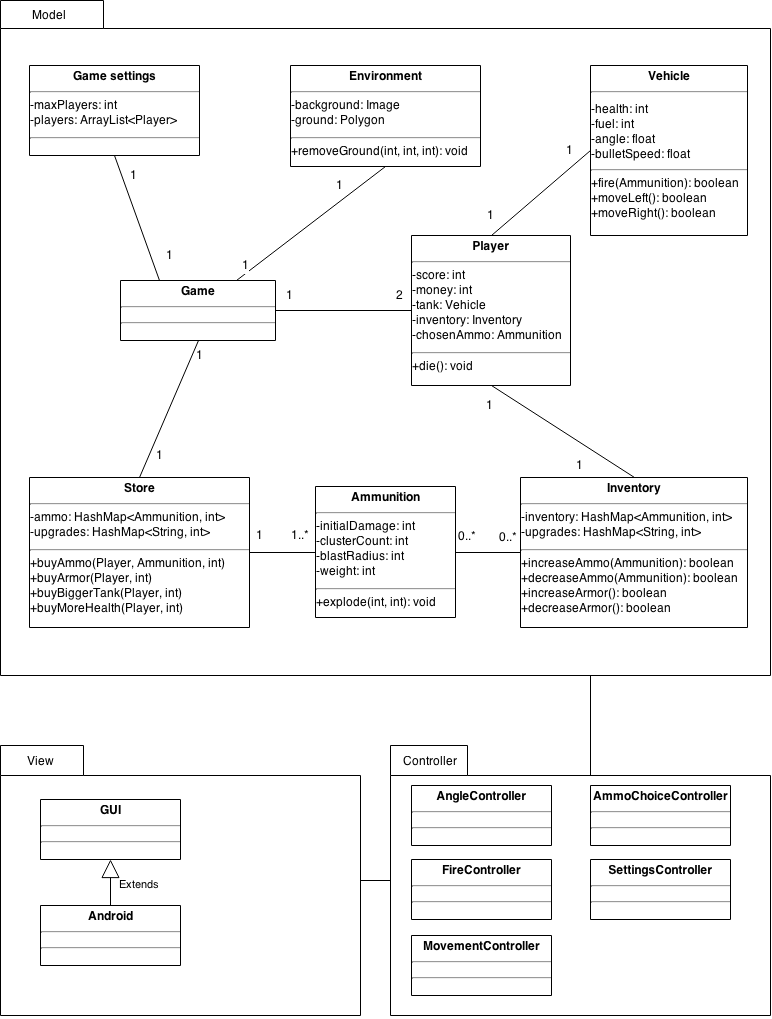
\includegraphics[scale=0.4]{images/logic_view.png}
\caption{Logic view}
\label{fig:logic-view}
\end{figure}

Our logic view (see Figure \ref{fig:logic-view}) is based on the logic view from The “4+1” View Model of Software Architecture \cite{krutchen}, but was built with a more recent modeling tool, UML. The modelling is also influenced by examples using the MVC-pattern from the lectures.

The logic view has been separated the different classes into the different parts of MVC. The model contains the classes which hold information about the game, such as game settings and players. These classes are specified with their most important fields and methods, e. g. a vehicle’s ability to fire or the initial damage of a certain ammunition type. It also covers the relationship between the classes, specifying which classes are connected and how many of these relations are allowed.
The controller simply contains the different controllers which will be used to change values in the model, based on what the user does in the view (GUI).
The view contains a GUI- and an Android-class, to illustrate that the view mainly consists of a GUI and that we wish to implement this GUI on a device running the Android OS. Implementing the GUI will be made easier by using the framework libGDX, but this is not shown in the view part, as libGDX will be utilized for other operations as well (e. g. game logic). 

As previously mentioned, we want to use libGDX to ease development. We have not included this in the logic view, as the full extent to which we will utilize libGDX is not decided, due to inexperience with the framework. 


\section{Process View}
\begin{figure}
\centering
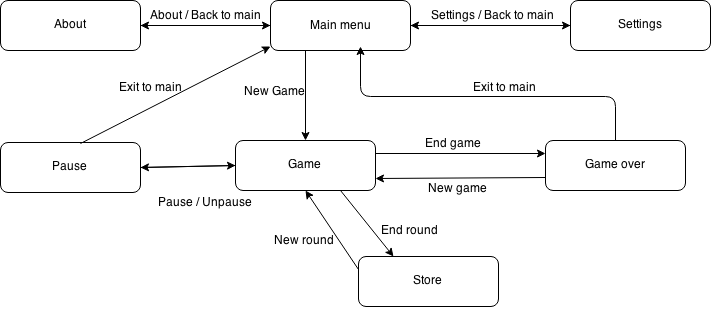
\includegraphics[scale=0.4]{images/process_view.png}
\caption{Process view}
\label{fig:process-view}
\end{figure}

Figure \ref{fig:process-view} shows the process view of the application. It is divided into the different scenes you will encounter when playing the game. You start at the “Main menu”. 

The double arrows symbolizes a splash screen that will be put on top of the scene you came from (e.g. when going from “Main menu” to “Settings”, the “Settings” scene will be put on top of “Main menu” and removed when abandoned.). A single arrow will remove the current scene and generate the subsequent.

When starting the game, you have a couple of choices: you can get information about the game (“how to play” and who developed it), change the settings or start a game with predefined settings. When playing the game, you can pause the game and from there end it. When a round is over, you will be presented with the store, where you can buy upgrades and ammunition. When this is done, you will start a new round. When the game is over (i.e. a player has won) you will be presented with two choices: you can either start a new game with the same settings, or you can exit the game and go to the main menu.


\section{Developement View}

\begin{figure}
\centering
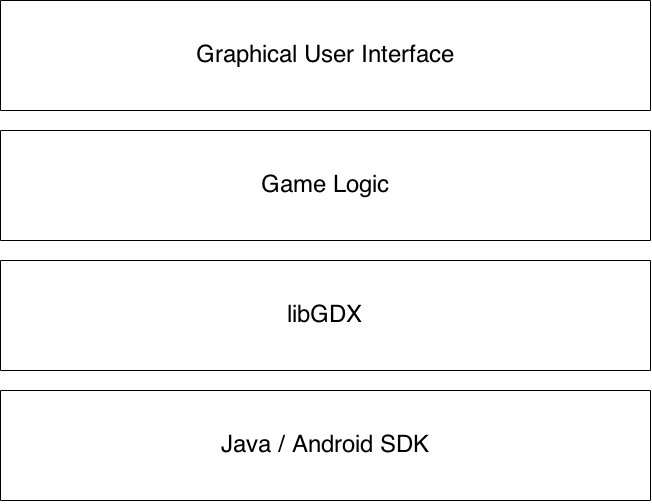
\includegraphics[scale=0.4]{images/development_view.png}
\caption{Development view}
\label{fig:development-view}
\end{figure}

The project is written in Java using the Android SDK. libGDX is the framework chosen for the game programming. These two gives us the foundation for writing our game logic and the game logic is used when writing the GUI. See Figure \ref{fig:development-view}.
